%% Adapted from `tikzposter-example.tex',

%% Modify the size of the paper for the usual 4 ft x3 ft poster size
\PassOptionsToPackage{paperwidth=48in, paperheight=36in,
  textwidth=48in, textheight=36in,
  innermargin=1in, margin=.25in,
  centering}{geometry}


\documentclass[25pt, landscape,blockverticalspace=0.5in, colspace=0.5in, subcolspace=0.33in]{tikzposter} %Default values for poster format options.

%% sans-serif fonts
\usepackage[scaled]{helvet}
\renewcommand\familydefault{\sfdefault} 
\usepackage[T1]{fontenc}
\usepackage[helvet]{sfmath}
\everymath={\sf}

%% arbitrary positioning
\usepackage[absolute,overlay]{textpos}

\usepackage[backend=bibtex,citestyle=numeric-comp]{biblatex}
\addbibresource{bibliography.bib} % bibliography file

\tikzposterlatexaffectionproofoff % remove tikzposter logo


 % Title, Author, Institute
\title{A most excellent research project}
\author{First Author$^1$, Second Author$^2$}
\institute{${}^1$ Clarkson, ${}^2$ Not Clarkson}


% -- PREDEFINED THEMES ---------------------- %
 % Choose LAYOUT:  Default, Basic, Rays, Simple, Envelope, Wave, Board, Autumn, Desert,
 \usetheme{Autumn}

 \definecolorpalette{Clarkson}{ % colors based on Clarkson visual identity guide
   \definecolor{colorOne}{HTML}{004E42}
   \definecolor{colorTwo}{HTML}{D7D2CB}   
   \definecolor{colorThree}{HTML}{FFCD00}
 }
\usecolorstyle[colorPalette=Clarkson]{Germany}


 \begin{document}

 \maketitle
 \node[anchor=west] at (TP@title.west) {\hspace{3in}
\includegraphics[height=3in]{logos/clarkson-seal.png}};
 \node[anchor=east] at (TP@title.east) {
\includegraphics[height=2in]{logos/clarkson-logo.png} \hspace*{2in}};


 \begin{columns}%blocks will be placed into columns

       \column{.33}

       \block{Title}{


         Math:
         \[
           \int_0^t f(x(\tau))d\tau 
         \]

         We can also put a graph in and refer to it here: Fig.~\ref{fig:first}
         \begin{tikzfigure}[This is a graph.]\label{fig:first}
           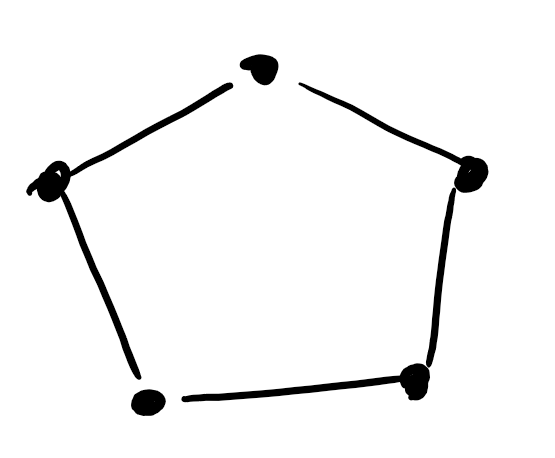
\includegraphics[width=0.5\linewidth]{figs/graph}
         \end{tikzfigure} 

       }


       \column{.33}

       \block{Methods}{
         Something common.

         \coloredbox{Important statement can be highlighted}
       }

     
       \begin{subcolumns}
         \subcolumn{.5}
         \block{Type 1}{
           Something cited from
           \cite{Hill1894}
         }
         \subcolumn{.5}
         \block{Type 2}{
           Something else}

       \end{subcolumns}

       \block{More}{
         For more information, take a look at \texttt{tikzposter-example.tex} and \texttt{tikzposter-example.pdf} in this folder. 
       }
       \note[targetoffsetx=2in, angle=-45,targetoffsety=0in,connection]{Additionally, documentation for the poster class is in \url{https://ctan.org/pkg/tikzposter}.}


       \column{.33}

       \block{Results}{
       }
       
       \block{References}{
         \printbibliography[heading=none]
       }

     \end{columns}



 \end{document}




\endinput
%%
%% End of file `tikzposter-example.tex'.
